\documentclass[10pt,a4paper]{article}
\usepackage[utf8]{inputenc}
\usepackage{amsmath}
\usepackage{amsfonts}
\usepackage{amssymb}
\usepackage{graphicx}
\author{Chelsea Sandridge, Paul Diaz, Sean Lopp, Colton Bryant, Kelsey Kalmbach}
\title{Modeling Ebola: SEIR Model, Computational Costs, and  Sensitivity in the Inverse Problem}
\begin{document}
\maketitle

\section*{Model}


\section*{Computational Costs}

Some sort of discussion on ode15s

\subsection*{Jacobian}


\subsection*{Speed Test}
A computational experiment was designed to test whether or not providing the Jacobian to ode15s increased the speed of the solver. This experiment consisted of the following steps:

\begin{enumerate}
\item Solve the system using ode15s with and without the Jacobian 1000 times. Take the mean time of the 1000 runs with the Jacobian, call this $y_1$. Similarly, take the mean time of the 1000 runs without the Jacobian, call this $x_1$.
\item Repeat step 1 30 times, giving a 30 by 1 vector $\mathbf{y}$ and a 30 by 1 vector $\mathbf{x}$.
\item Calculate the paired difference $d_i =x_i - y_i$ for each $i$, or equivalently $\mathbf{d=x-y}$. Note that $d$ will be positive if the solver was faster with the Jacobian provided.
\item The vector $\mathbf{d}$ can be used to test the hypothesis
$ H_o: D <= 0$ where $D$ is the test statistic:
$$ \frac{\bar{d}}{s/\sqrt{n}} \sim t_{n-1}(0,1)$$
where $\bar{d}$ is the mean of the paired differences, $s$ is the  sample standard deviation of the paired differences, $n=30$, and $t_{n-1}$ is the student's t-distribution with $n-1$ degrees of freedom. If we reject the null hypothesis than there is significant evidence that the solver is faster with the Jacobian provided.
\end{enumerate}

The test is conducted in this way to account for differences in solve time that depend on computer performance which can vary at any given time. Figure ~\ref{fig:speedtest} depicts the result of this experiment run on a Windows computer with 4GB of RAM and an i3 processor.

\begin{figure}[!ht]
\centering
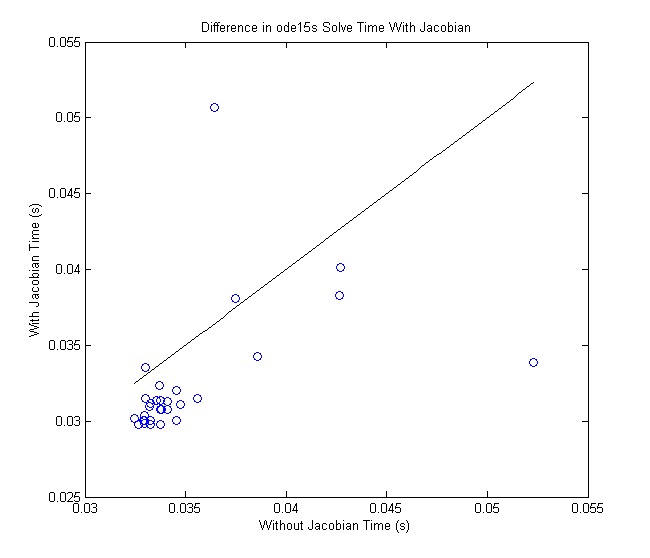
\includegraphics[scale=0.6]{speedtest}
\caption{Results of the speed test indicate the solver is faster with the Jacobian provided. Additionally, the outlier points demonstrate the need to clock more than one code execution}.
\label{fig:speedtest}
\end{figure}

The final p-value was 0.0014, which leads us to reject the null hypothesis and conclude that there is statistical evidence that the solver runs faster with the Jacobian provided.


\section*{Sensitivity in the Inverse Problem}

The model parameters were fit based on data using an optimization algorithm. However, there is uncertainty in this process.  For example, how reliable are death and infection numbers reported from an African country? The reported data can be thought of as a sample from the true underlying process. Another source of uncertainty is the amount of data. For example, a model fit with data from one country will have different parameters than a model fit with data from multiple countries. This is analogous to sample size.

We used Markov Chain Monte-Carlo (MCMC) to study the impact of uncertainty on the parameter values. First, a set of parameters was taken as ``truth". Test data was then generated from this ``true" model. This test data was used to create sample data sets of different sizes. Then random noise, $\epsilon \sim N(0,s)$, was added to the sample data sets. Next, MCMC was used to estimate the distribution of $\beta_0, \beta_1$ and $\beta_3$ based off of these different sample data sets. In our case, only the number of dead people was used as test data, as this number is the most likely to be reported and also the most likely to have high amounts of uncertainty.

\subsection*{MCMC}

The theory behind MCMC is that the parameter distribution for a function given data, $\mathbf{\theta}|y=f(\theta,x)$, will be the steady-state distribution of some Markov Chain. Because the parameter distribution depends on the data it is called a posterior distribution. To approximate the posterior for the parameter one can sample repeatedly from this Markov Chain (this random sampling is the Monte-Carlo part). In practice this is done using the Metropolis-Hastings algorithm:

\begin{enumerate}
 \item Start with an initial guess for the parameters and calculate $\hat{y_0}=f(\theta_0,x)$. Compute the residuals $e_0=||\hat{y_0}-y||$. 
 
 \item Take a random step away from your initial guess for the parameters. Calculate the new estimates, $\hat{y_1}=f(\theta_1,x)$ and residuals residuals $e_1=||\hat{y_1}-y||$.
 
 \item Compute the likelihood ratio that compares the fit of the estimates from the original model to the estimates of the new model, $f(e_1,e_2)$. Typically the errors $e_0$ and $e_1$ are assumed to be normally distributed with equal variance in which case the likelihood ratio is $$\exp[(-e_1+e_2)/2\sigma^2]$$. 
 
 \item Now, if the likelihood ratio is greater than 1 then the data was more likely to have come from the new parameters. In this case the new parameters become the new guess and we return to step 1.   If the likelihood ratio is less than 1 than a decision needs to be made. The natural thing to do would be to reject the new parameters, and to try taking a random step in another direction away from $\theta_0$. However, it turns out that if this is done all the time the entire parameter space will not be effectively searched. (Meaning that we will not have appropriately sampled from the distribution of the Markov Chain). To fix this problem we sometimes accept the new parameters even when the likelihood ratio is less than 1. Specifically, we draw a random number that is distributed uniformly across the interval (0,1). If the likelihood ratio is greater than this random number, we accept the new parameters.
 
\end{enumerate}

Implemented in this way, MCMC allow us to efficiently take a random walk across the parameter space in such a way that our samples converge on the parameter distribution (brilliant!). Usually the fist portion of samples is discarded, and the remaining samples can be used to estimate quantities of interest. For example, $E[\theta]=\bar{\theta}$.

\subsection*{Results}


Table ~\ref{tab:mcmctable} presents the results of the MCMC experiment. The ``true" parameter values were $\beta_1=2e-8$, $\beta_2=2e-9$, and $\beta_3=2e-9$. The data generating process given these parameters is depicted in Figure ~\ref{fig:mcmctrue}. Interestingly, it appears that sample size has a bigger influence on the posterior distribution than the amount of noise added to the sample data. The variances of the distribution appear to be stable, with a somewhat increasing trend for smaller sample sizes and large noise. The bias in the posterior was different for each parameter. While the posterior distribution for $\beta_0$ and $\beta_3$ was almost always centered around the true value significant bias was introduced for $\beta_2$. Finally, for the most difficult experiment with a small sample size $n=25$ and large noise $s=10$ the sampling chain did not converge. This is apparent in Figure~\ref{fig:mcmcnoconverge} where the chains have significant trend. In contrast, Figure ~\ref{fig:mcmcoutput} demonstrates the distribution and sampling chain for a convergent MCMC experiment.

\begin{figure}
\centering
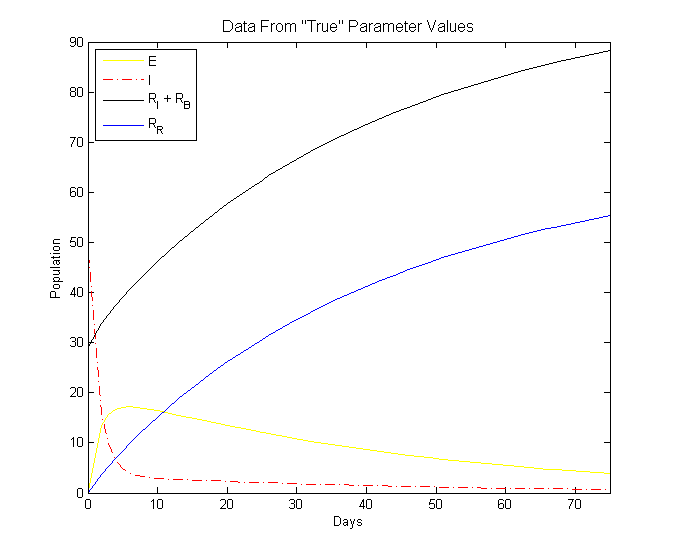
\includegraphics[scale=0.6]{truth}
\caption{Model outputs assuming the ``true" parameter values of $\beta_1=2e-8$, $\beta_2=2e-9$, and $\beta_3=2e-9$}
\label{fig:mcmctrue}
\end{figure}

\begin{table}
\centering
\noindent\makebox[\textwidth]{%
\begin{tabular}{rr|rrrrrr}
\hline
Sample Size & Noise $\sim N(0,s^2)$& $\bar{\beta_1}$ & $\bar{\beta_2}$ & $\bar{\beta_3}$ & $SD(\hat{\beta_1})$ & $SD(\hat{\beta_2})$ & $SD(\hat{\beta_3})$ \\
\hline
25 & 0 & 1.83e-8 & 5.49e-9 & 2.16e-9 & 4.98e-10 & 5.04e-10 & 4.97e-10 \\
50 & 0 & 1.99e-8 & 2.01e-9& 2.00e-9 & 5.17e-10 & 5.60e-10 & 4.99e-10 \\
25 & 5 & 2.00e-8 & 7.02e-9 & 1.82e-9 & 5.28e-10 & 6.16e-10 & 5.00e-10 \\
50 & 5 & 1.55e-8 & 4.40e-9 & 2.59e-9 & 5.01e-10 & 5.04e-10& 4.96e-10\\
25 & 10 & na & na & na & na & na & na \\
50 & 10 & 2.01e-8 & 2.99e-9 & 2.11e-9 & 5.077e-10 & 5.23e-10 & 5.01e-10 \\
\hline
\end{tabular}
}
\caption{Results of MCMC for different sample sizes and different random noise}
\label{tab:mcmctable}
\end{table}

\begin{figure}
\centering
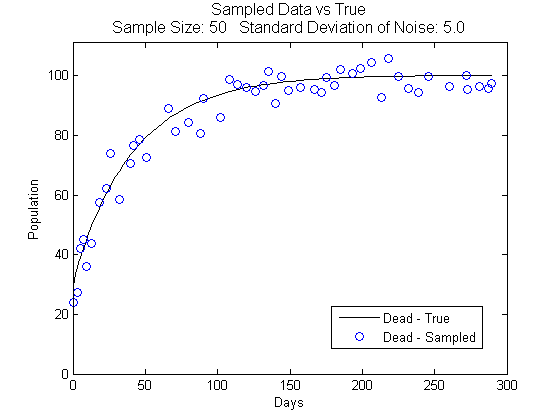
\includegraphics[scale=0.6]{noisydata}
\caption{An example of the noisy data set compared to the ``true" data generating process.}
\label{fig:noisydata}
\end{figure}

\begin{figure}
\centering
\noindent\makebox[\textwidth]{%
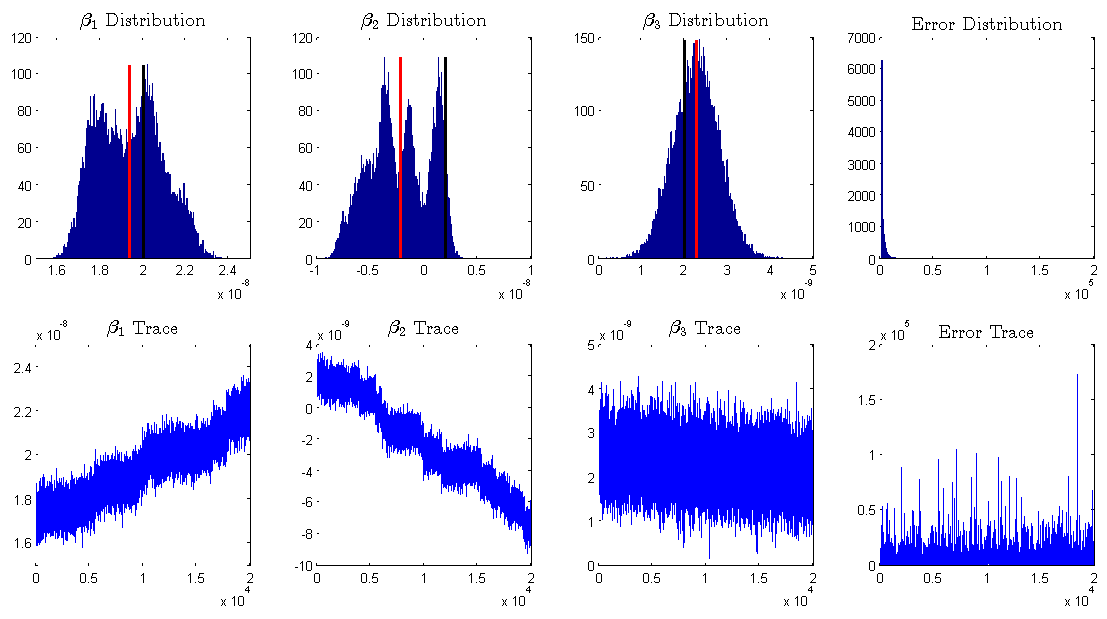
\includegraphics[scale=0.6]{mcmcnoconverge}
}
\caption{For the experiment $s=10$ and $n=25$ the sampling chain did not converge.}
\label{fig:mcmcnoconverge}
\end{figure}


\begin{figure}
\centering
\noindent\makebox[\textwidth]{%
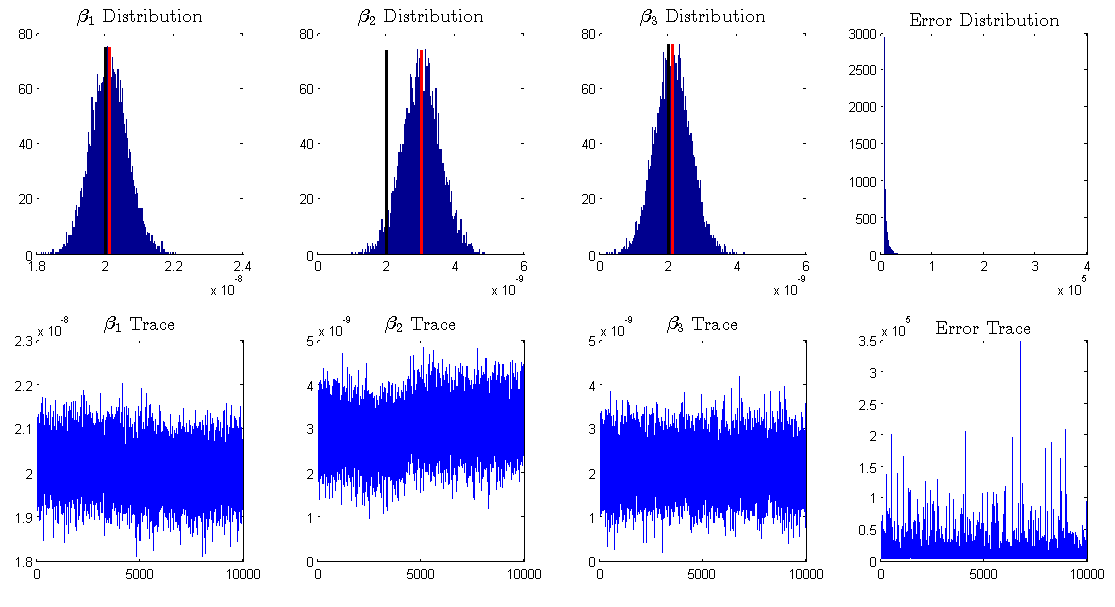
\includegraphics[scale=0.6]{mcmcoutput}
}
\caption{An example of the results of MCMC. Top: Each estimated distribution of the parameter with the true value for the parameter (black) and the distribution mean (red). Also included is the distribution for the error $e=||\hat{y}-y||$ where $\hat{y}=f(\hat{\beta1},\hat{\beta2},\hat{\beta3})$. Bottom: The MCMC sampling chain. For a convergent MCMC this should look like a solid black band. Drift or oscillatory bands suggest that the MCMC did not converge to the posterior distribution of the parameter.}
\label{fig:mcmcoutput}
\end{figure}


\end{document}